\section{Resultat}
\label{sec:joel_o-results}
Från de beskrivna metoderna har en mängd resultat sammanställts för att ge svar på frågeställningarna. Analysen av Javascript-projekt har givit en stor mängd kvantitativa resultat. Informationsundersökningen och projekterfarenheter erbjuder resultat av mer kvalitativ typ.

\subsection{Kvantitativa resultat}
\label{sec:joel_o-results-kvant}
Den 6 april 2018 passade 6743 Javascript-projekt på GitHub in på tidigare nämnda definition av populära projekt. Av dessa innehöll 5~402, 80.1\% en \texttt{package.json} fil och ansågs därför vara av intresse för undersökningen. Samtliga data som presenteras här är baserade på dessa 5~402 projekt. Totalt hittades 114~249 beroenden varav 991, 0.87\% refererade till paket utanför npm-systemet.

De värden som är av intresse är projekts direkta beroenden, indirekta beroenden samt det maximala djupet på beroendekedjor. Medelvärde ($\bar{x}$), standardavvikelse ($\sigma$) och maxvärde ($x_{max}$) för dessa finns presenterade i tabell \ref{tab:beroende-data}. Minvärdet för samtliga är 0.

\begin{table}
  \centering
  \begin{tabular}{c | c c c | c c c | c c c |}
    \cline{2-10}
    & \multicolumn{3}{c|}{Direkta Beroenden} & \multicolumn{3}{c|}{Indirekta Beroenden} & \multicolumn{3}{c|}{Beroendedjup} \\ \cline{2-10}
    & $\bar{x}$ & $\sigma$ & $x_{max}$ & $\bar{x}$ & $\sigma$ & $x_{max}$ & $\bar{x}$ & $\sigma$ & $x_{max}$ \\ \hline
    \multicolumn{1}{|c|}{\textit{dependencies}} & 6.76 & 12.5 & 153 & 95.02 & 200.21 & 1779 & 4.34 & 4.90 & 24 \\ \hline
    \multicolumn{1}{|c|}{\textit{devDependencies}} & 14.21 & 15.47 & 135 & 466.07 & 384.91 & 2202 & 10.42 & 5.71 & 21 \\
    \hline
  \end{tabular}
  \caption{Medelvärden, standardavvikelser och maxvärden för undersökta värden}
  \label{tab:beroende-data}
\end{table}

\begin{figure*}
    \centering
    \begin{subfigure}[]{0.5\textwidth}
        \centering
        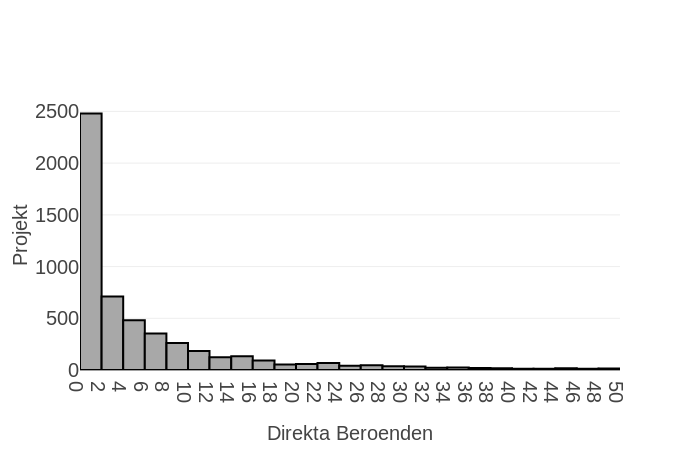
\includegraphics[height=5cm]{direct_dep}
        \caption{\textit{dependencies}}
    \end{subfigure}%
    ~
    \begin{subfigure}[]{0.5\textwidth}
        \centering
        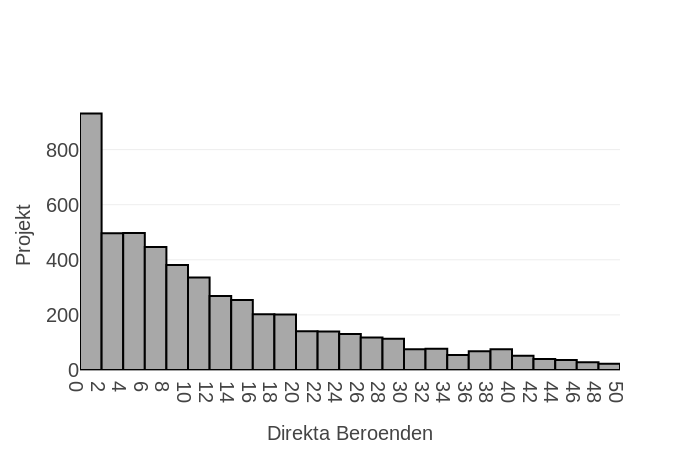
\includegraphics[height=5cm]{direct_dep_dev}
        \caption{\textit{devDependencies}}
    \end{subfigure}
    \caption{Histogram över projekt med maximalt 50 direkta beroenden}
    \label{fig:direct-dep}
\end{figure*}

Histogram över antalet beroenden presenteras i figur \ref{fig:direct-dep}. Av de analyserade projekten hade 1853, 27.50\% inga beroenden. Samma siffra för \textit{devDependencies} är betydligt lägre på endast 696 projekt, 12.90\% med inga beroenden för utveckling. Från histogrammen syns det tydligt att den största gruppen av projekt har inga eller endast några få beroenden. För \textit{dependencies} avtar mängden projekt hastigt för större antal beroenden. \textit{DevDependencies} visar inte en lika snabb nedgång för större antal beroenden. Här visar histogrammet en mer jämn uppdelning och först framåt 20 beroenden börjar mängderna projekt kraftigt avta.

\begin{figure*}
    \centering
    \begin{subfigure}[]{0.5\textwidth}
        \centering
        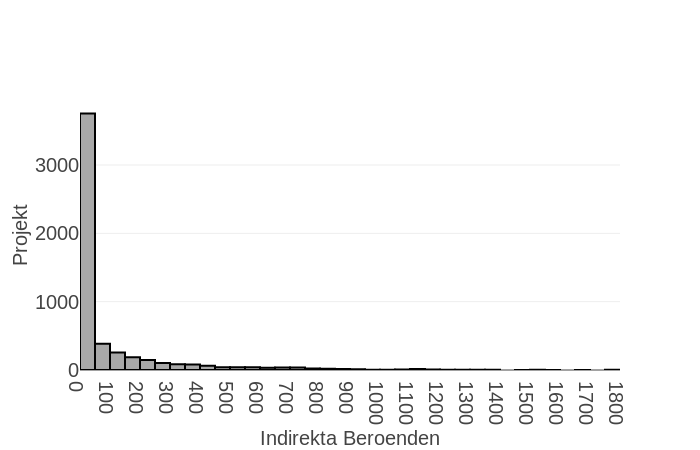
\includegraphics[height=5cm]{indirect_dep}
        \caption{\textit{dependencies}}
    \end{subfigure}%
    ~
    \begin{subfigure}[]{0.5\textwidth}
        \centering
        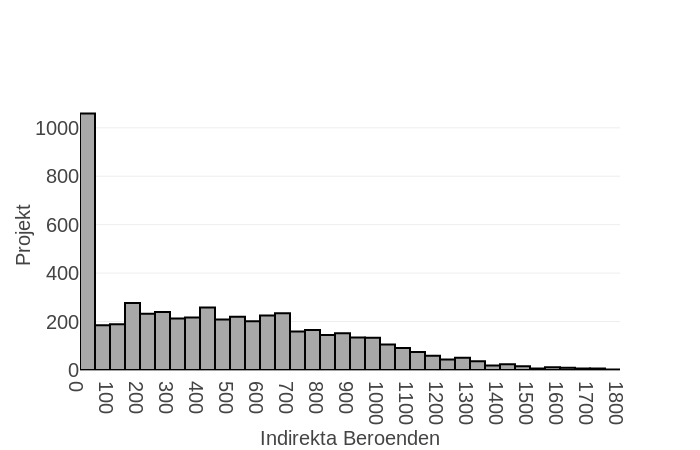
\includegraphics[height=5cm]{indirect_dep_dev}
        \caption{\textit{devDependencies}}
    \end{subfigure}
    \caption{Histogram över projekt med maximalt 1800 indirekta beroenden}
    \label{fig:indirect-dep}
\end{figure*}

En liknande fördelning över \textit{dependencies} syns för indirekta beroenden i figur \ref{fig:indirect-dep}. Här är dock antalet \textit{devDependencies} mycket utspritt. Förutom den stora mängd med inga eller några få indirekta beroenden finns en något jämn fördelning mellan 100-700 beroenden. Detta betyder att det finns en substantiell mängd projekt med flera hundra indirekta beroenden för utveckling.

\begin{figure*}
    \centering
    \begin{subfigure}[]{0.5\textwidth}
        \centering
        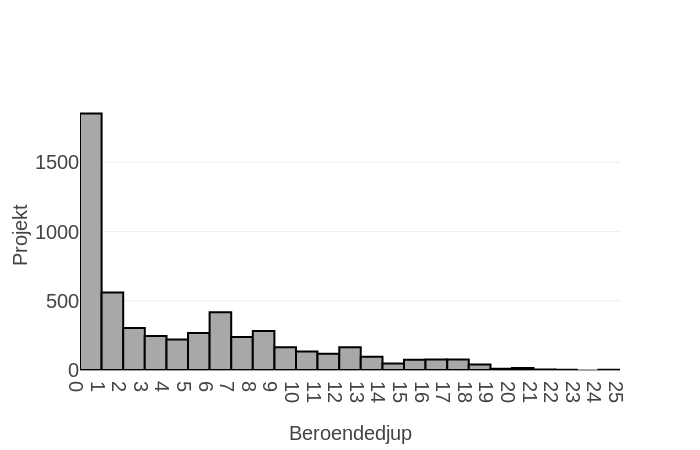
\includegraphics[height=5cm]{dep_depth}
        \caption{\textit{dependencies}}
        \label{fig:dep-depth-dependencies}
    \end{subfigure}%
    ~
    \begin{subfigure}[]{0.5\textwidth}
        \centering
        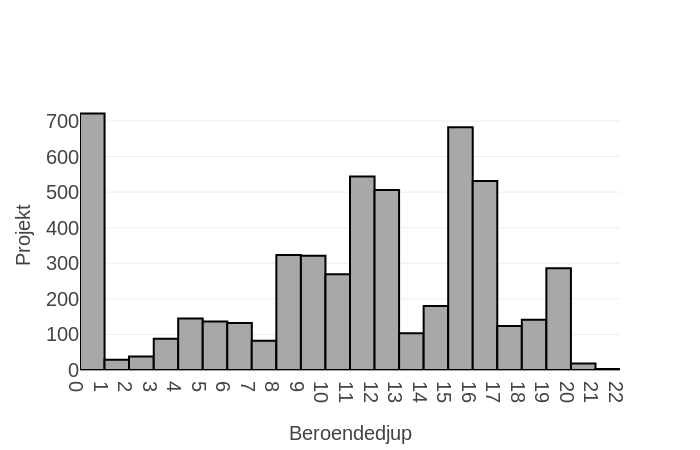
\includegraphics[height=5cm]{dep_depth_dev}
        \caption{\textit{devDependencies}}
        \label{fig:dep-depth-devDependencies}
      \end{subfigure}
    \caption{Histogram över projektens beroendedjup}
    \label{fig:dep-depth}
\end{figure*}

Även djupet av beroenden är mycket större för \textit{devDependencies}, även om det maximala djupet av 24 i tabell \ref{tab:beroende-data} är för \textit{dependencies}. I histogrammet \ref{fig:dep-depth-dependencies} syns en liknande fördelning av djup som för antal beroenden. En dominerande del av projekten saknar beroenden, här dock med en något jämn fördelning av projekt med 2 till 9 nivåer. För \textit{devDependencies} syns dock en spretig uppdelning i figur \ref{fig:dep-depth-devDependencies}. Även om många projekt har 0 beroendenivåer finns här nästan lika stora mängder runt djup 12 och 16. Det är tydligt att det är mycket vanligt att Javascript-projekt har \textit{devDependencies} som sträcker sig många nivåer genom npm-systemet.

\subsection{Påverkan på utvecklingsprocessen}

Färdiga paket har under det genomförda projektet erbjudit många möjligheter. Det stora ramverket React har varit centrala för utvecklingen av användargränssnitt och interaktion. Speldelen av projektet har även kunnat förenklats genom användandet av paketet PixiJS. Flera paket har även varit centrala för utvecklingsarbetet. Speciellt paket för testning har erbjudit automatisering som inte hade varit möjlig utan dessa. Det är ej troligt att kodens kvalitet till samma grad hade kunnat garanterats genom projektet utan dessa verktyg.

Att arbeta med färdiga paket tycks även till viss del förändra vad som krävs av utvecklare. När paket adderades till projektet var det viktigaste att dessa integrerades korrekt. Detta krävde kunskap om paketen som användes och om hur de skulle passa in i systemet som utvecklades. Här spelar utvecklarens tidigare vana av paketen samt dokumentation en stor roll. Detta är till viss del skillt från egenskaper som logiskt tänkande och algoritmisk problemlösning som annars associeras med mjukvaruutveckling.

Att i utvecklingsarbete integrera flera färdiga paket har visat sig även skapa en något ökad osäkerhet i felsökning. Det har i det genomförda projektet uppkommit situationer då det inte är klart om buggar beror på den egna koden, kod i importerade paket eller en felaktig integration av paket. Dessa ovissheter ökar med ovetskapen om paketen som arbetas med.

Datan från undersökningen av Javascript-projekt visar att hjälppaket för utvecklingsarbetet används i stor utsträckning. Dessa paket har ofta flera beroenden under sig, vilket leder till ett utvecklingsarbete som vilar på att stora mängder paket fungerar korrekt. S. Scott Henry har studerat en problematisk förändring till paketet \textit{mkdirp} som ofta användes i utvecklingsprocesser.\cite{Henry2017} Denna förändring skapade stora problem för utvecklare som använde den nya versionen, men problemen åtgärdades mycket snabbt. Exemplet visar på hur paket som är centrala för utvecklares arbete är kritiska för utvecklingsproccessen, men också att problem som direkt når utvecklare löses mycket effektivt.

\subsection{Påverkan på säkerhet och tillförlitlighet}
Inkludering av färdiga paket ökar mängden kod i projekt och därmed möjliga problem med säkerhet och tillförlitlighet. Att paket oftast är publicerade som open-source och används i många olika projekt är dock anledningar att tro att denna kod har en hög kvalitet.\cite{coverity-scan2013}

Det finns trots detta flera exempel där säkerhetsproblem har förekommit i npm-paket och genom beroenden påverkat andra paket och projekt. Joseph Hejderup utförde 2015 en undersökning av dessa problem.\cite{Hejderup2017} De vanligaste problemen i npm-paket har visat sig vara känslighet för attacker som \textit{cross site scripting} och \textit{denial of service}(då Javascript används som server-språk). Hejderup identifierade i sin undersökning över 1500 paket med beroenden till paket med säkerhetsproblem. En grov uppskattning gav att ungefär 1\% av npm-ekosystemet kunde vara i riskzonen för kända säkerhetsproblem.

I tidigare nämnda arbete poängteras också att utvecklare till paket ofta inte visat någon medvetenhet över säkerhetsproblem i beroenden. Detta beror möjligen på att många paket är utdaterade och inte längre underhålls kontinuerligt. Denna observation visar på vikten för utvecklare att ha en stor medvetenhet om hur pass uppdaterade integrerade paket är. För att kunna garantera säkerhet i Javascript är det troligen nödvändigt att till viss del vara insatt i problem och underhåll för de paket som beroenden finns till.

En större kodmängd av jämn kvalitet leder till större chans för buggar och en lägre tillförlitlighet. Vid inkludering av färdiga paket kan kod dock förväntas hålla en högre kvalitet jämfört med egenproducerad kod. Erfarenheter från det gångna projektet visar att introducerade problem mycket sällan kommer från buggar i de integrerade paketen. Ofta kommer problemen istället från felaktig integration och använding av paketen.

I de fall fel uppstår på grund av inkludering av färdiga paket (antingen direkt i paketen eller i integrationen) påverkas även systems tillförlitlighet av mängden resurser som finns för reparation av mjukvaran. God dokumentation och större mängder utvecklare med kunskap av arbete med vissa paket gör att problem kan förväntas lösas enklare jämfört med egenproducerad kod. Detta förkortar MTTR och minskar den tid system kan förväntas vara otillgängliga.
